\section{Descripción del sistema}

El proceso de consulta psicológica inicia cuando el paciente se decide por obtener apoyo del psicólogo, lo cual empieza con programar una cita para realizar su consulta psicológica, el psicólogo revisa la disponibilidad en su agenda, al encontrar un espacio para atender al paciente le hará saber el día y hora en la cual lo puede atender, si el paciente no tiene inconveniente se agenda la cita. Al llegar la fecha y hora indicada el paciente se presenta en el consultorio, en este momento se detecta si es un paciente nuevo o ya tiene un expediente con el psicólogo, al no tener un expediente se generará uno nuevo, el paciente proporcionará información médica y personal para completar el expediente; si el paciente ya contaba con un expediente se continua con las sesiones psicológicas donde se pueden aplicar pruebas psicológicas de distintos tipos, de igual forma un paciente nuevo al completar el proceso de creación de expediente pasa a la etapa de realizar pruebas psicológicas. Las respuestas y resultados obtenidos de estas pruebas son registradas por el psicólogo para posteriormente ser analizadas por el mismo y generar el informe psicológico que le será entregado al paciente.
Al entregar el informe se termina el proceso de consulta psicológica con lo que se queda en espera de agenda una nueva cita.

\begin{figure}[H]
\centering
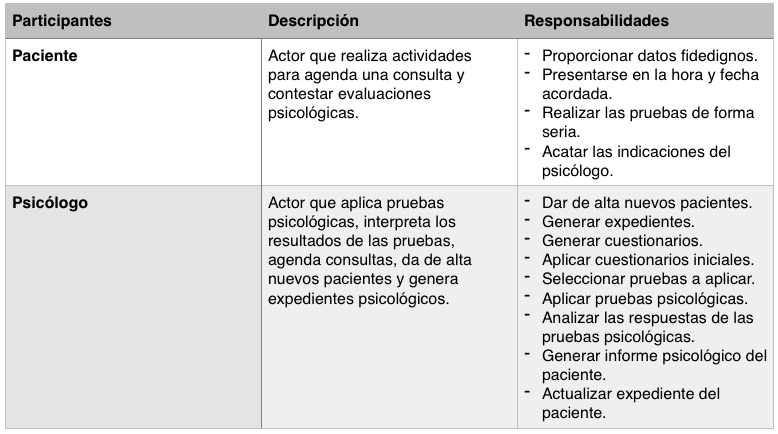
\includegraphics[width=\textwidth]{imagenes/actores}
\caption{Descripción de los actores implicados}
\label{img:actores}
\end{figure}

\subsection{Diagrama del proceso}

\begin{figure}[H]
\centering
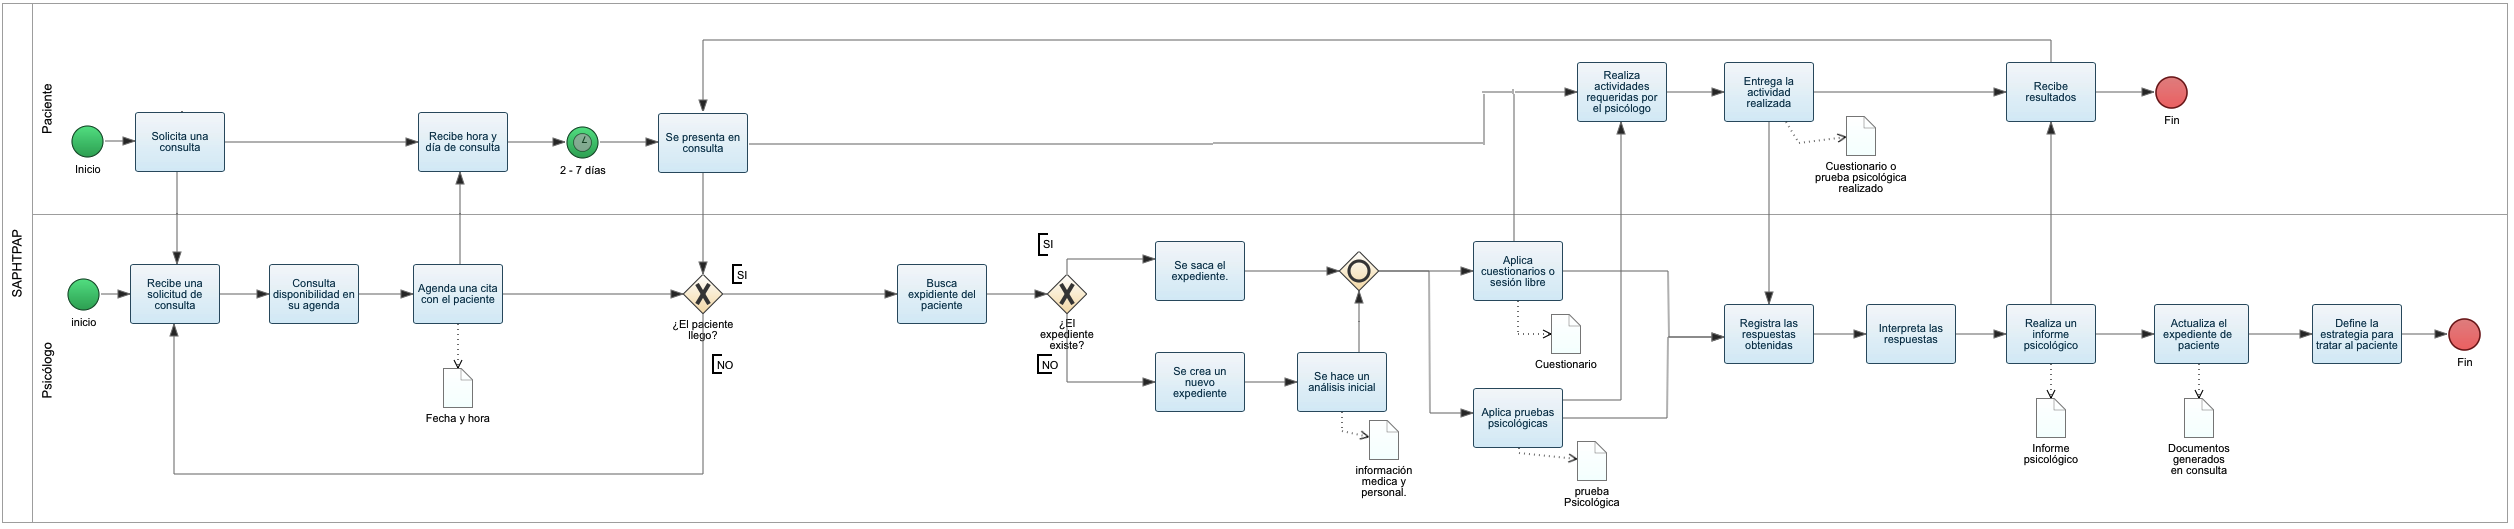
\includegraphics[width=\textwidth]{imagenes/PFinal}
\caption{Proceso Actual}
\label{img:proces1}
\end{figure}
\newpage
\subsection{Diagrama del proceso por secciones}

\begin{figure}[H]
\centering
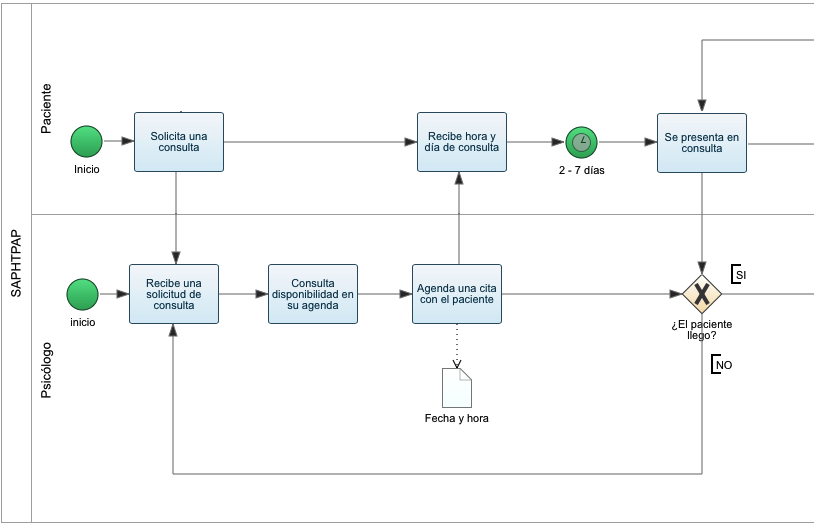
\includegraphics[width=0.8\textwidth]{imagenes/PFinal_1}
\caption{Sección 1 del proceso}
\label{img:proces1_1}
\end{figure}

\begin{figure}[H]
\centering
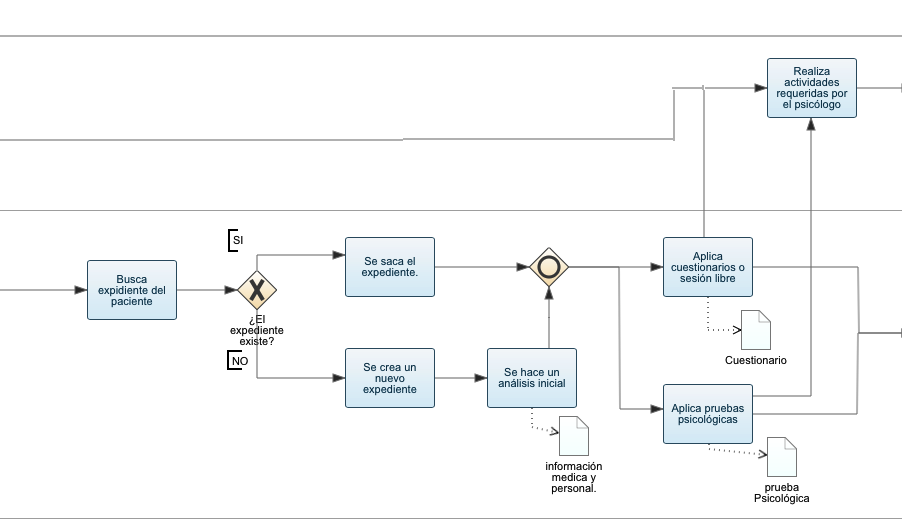
\includegraphics[width=0.8\textwidth]{imagenes/PFinal_2}
\caption{Sección 2 del proceso}
\label{img:proces1_2}
\end{figure}

\begin{figure}[H]
\centering
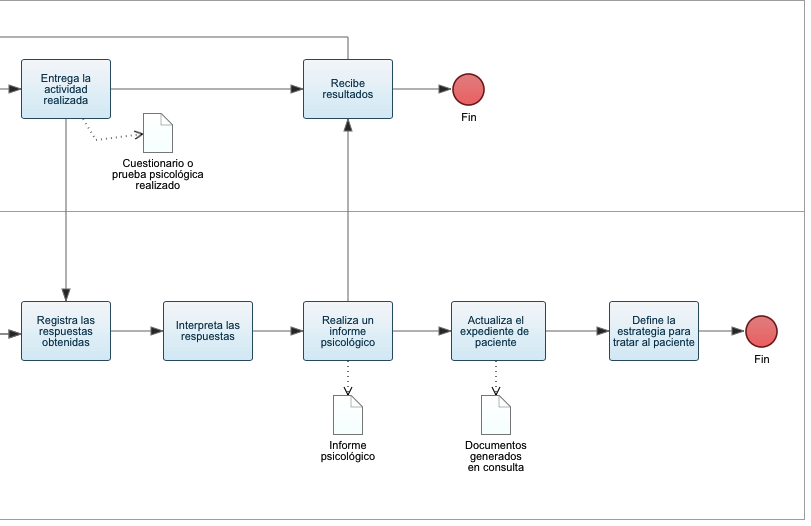
\includegraphics[width=0.8\textwidth]{imagenes/PFinal_3}
\caption{Sección 3 del proceso}
\label{img:proces1_3}
\end{figure}

\newpage